 \begin{center}
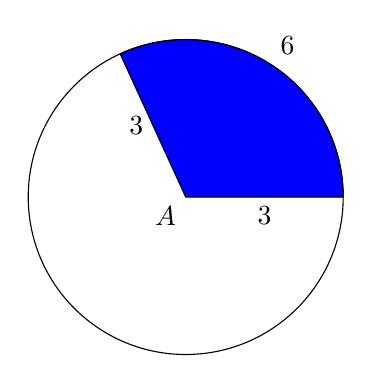
\begin{tikzpicture}
\draw(0,0)circle(2)node[anchor=north east]{$A$};
\fill[draw=black,fill=blue](0,0)--(2,0)arc(0:114.59:2)--cycle;
\draw(1,0)node[anchor=north]{$3$}(114.59:1)node[anchor=east]{$3$};
\draw(57.3:2)node[anchor=south west]{$6$};
\end{tikzpicture}\end{center}
The sector of circle $A$ above is bounded by two radii of length $3$ and an arc of length $6$.  What is the sector's area?


\ifsat
	\begin{enumerate}[label=\Alph*)]
		\item {\Large$\frac{\pi}{4} $ }
		\item $4 $ 
		\item $9 $ % 
		\item $9\pi  $
	\end{enumerate}
\else
\fi

\ifacteven
	\begin{enumerate}[label=\textbf{\Alph*.},itemsep=\fill,align=left]
		\setcounter{enumii}{5}
		\item {\Large$\frac{\pi}{4} $ }
		\item $4 $ 
		\item $9 $ % 
		\addtocounter{enumii}{1}
		\item {\Large$\frac{9\pi}{2} $ }
		\item $9\pi  $
	\end{enumerate}
\else
\fi

\ifactodd
	\begin{enumerate}[label=\textbf{\Alph*.},itemsep=\fill,align=left]
		\item {\Large$\frac{\pi}{4} $ }
		\item $4 $ 
		\item $9 $ % 
		\item {\Large$\frac{9\pi}{2} $ }
		\item $9\pi  $
	\end{enumerate}
\else
\fi

\ifgridin
 $9 $ % 
		
\else
\fi

